\section{ICBA and the Recovery Hierarchy}
\label{sec:auditor}

\subsection{The Audit Contract}
ICBA leaves graph construction and native traversal unchanged. Its input declares source and target snapshots, implementation, query population, action grid, permitted observations, failure event, and reference. Its output records raw reuse, candidate construction, certification counts and bounds, fallback, held-out risk, serving cost, and acquisition cost.

Selection, certification, and evaluation have disjoint roles. Selection may construct a policy. Certification checks frozen candidates and fallback; it cannot retrain or reorder them. Evaluation measures the completed decision and has no feedback path. If no action qualifies, the audit abstains. Raw reuse remains visible even when certification rejects it, so endpoint fallback cannot erase portability failure.

\subsection{A Least-Complexity Policy Ladder}
The recovery comparison is ordered by information and complexity:
\begin{enumerate}
\item a fixed native action, certified on target queries;
\item a target-global action selected and certified with target labels;
\item TCP, which retains a per-query historical profile and selects one target shift;
\item source-derived slack, retained as a portability diagnostic and ablation.
\end{enumerate}
Every candidate enters the same candidate--certificate--fallback interface. This makes a simpler passing policy evidence against the necessity of a more complex one.

\subsection{TCP: History Pooling Followed by One Target Shift}
\label{sec:tcp-implementation}
TCP uses native HNSW actions
\begin{equation}
 \mathcal A=(10,20,40,80,120,160,200).
 \label{eq:tcp-grid}
\end{equation}
For query $q$ and old build $g$, let $\tilde j_g(q)$ be the first-passing grid index, with unresolved labels retained at the endpoint. For target seed $t$, pool the nine other old builds:
\begin{equation}
 j_0^{(t)}(q)=\max_{g\in\mathcal H_t}\tilde j_g(q),\qquad
 \pi_s(q)=a_{\min\{j_0^{(t)}(q)+s,J\}}.
 \label{eq:shift}
\end{equation}
TCP applies to recurring profiled queries. Target selection scans shifts in ascending order and freezes the first shift whose selection-role CP bound passes. Candidate and endpoint then receive disjoint certification and held-out evaluation. Storing the profile costs $O(Q)$; acquisition is charged separately from serving lookup.

The original replay checks candidate and endpoint at $\alpha=.05$ each. The stricter frozen-response analysis assigns $\alpha_c=\alpha_e=.025$, applies the candidate-first order, and abstains if neither qualifies. This instantiates Proposition~\ref{prop:simultaneous} per target under its query-sampling assumptions. It is reported as a sensitivity because the confidence allocation was changed after the original replay.

\begin{figure*}[t]
\centering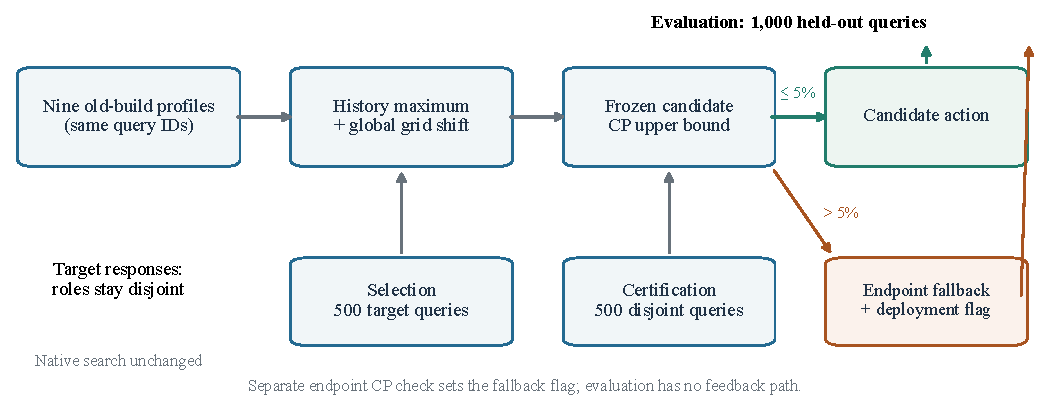
\includegraphics[width=\textwidth]{figures/workflow.pdf}
\caption{ICBA applied to a recurring-query policy. Historical profiles construct candidates; target selection freezes one rule; certification chooses candidate, endpoint, or abstention; evaluation has no feedback path. The same interface also accepts fixed and target-global candidates.}
\label{fig:workflow}
\Description{Historical response profiles feed a candidate construction stage, followed by disjoint target selection, certification, and evaluation roles.}
\end{figure*}

\subsection{Source-Derived Slack as an Ablation}
\label{sec:slack-method}
A source-design role chooses the lowest native action whose Bonferroni-adjusted CP bound passes and then shifts it upward by one grid rung, clipping at the endpoint. Later source certification and target evaluation roles are disjoint. The rule uses no target selection, so it isolates whether source evidence leaves recoverable slack. A subsequent target-certified stage freezes that candidate before new certification and evaluation roles are accessed. S9-4 compares it with fixed-256 and target-global policies on exactly the same prospective indexes and query roles. Its status is determined by that comparison, not by its absolute gain alone.
